\documentclass[12pt]{beamer}

\usepackage{amsmath}
\usepackage{float}
\usepackage{graphicx}
\usepackage[utf8]{inputenc}

\mode<presentation>{\usetheme{CambridgeUS}}
\title{Difracción de Franhaufer modelada por la Transformada de Fourier}
\author{Alfredo Ricci y Juan Andrés Urrea}

\begin{document}
%La portada
\frame{\titlepage}
%Así se comienza cada diapositiva
\begin{frame}
\frametitle{Aspectos a Desarrollar}
\begin{block}{}
\begin{enumerate}
\item Introducción y Marco Teórico
\item Metodología
\item Simulaciones Preliminares
\item Montaje Realizado
\item Datos Recolectados y Análisis 
\item Conclusiones
\end{enumerate}
\end{block}
\end{frame}

%La introducción
\begin{frame}
\frametitle{Introducción}
\begin{block}{}
\begin{itemize}
\item Se elige este tema por interés del grupo, tanto en el aspecto matemático como herramienta como en la visualización experimental de este.
\item El éxito representa una manera didáctica de combinar abstracciones matemáticas con fenómenos observables. Significa entonces poder visualizar la teoría más allá del "tablero", en la realidad.
\item Aún más específicamente, convierte la transformada de Fourier de un operador que aparenta ser abstracto a un fenómeno real y observable.
\end{itemize}
\end{block}
\end{frame}

%Marco Teórico
\begin{frame}
\frametitle{Marco Teórico}
\begin{block}{Base Matemática}
\begin{itemize}
\item T.F Función Continua Finita: $F(\omega)=\int_{a}^{b} f(t)e^{-2\pi i \omega t}dt$
\item Integral de Difracción Fresnel-Kirchoff: $U(P)=-\frac{Ai}{\lambda}\frac{\cos \delta}{r\prime s\prime}\int \int_C\frac{e^{ik(r+s)}}{rs}[cos(n,r)-cos(n,s)]dS $
\item Difracción de Fraunhaufer: $U(p,q)=\int \int_C G(\eta,\zeta) e^{-i\frac{2\pi}{\lambda}(p\zeta + q\eta)}d\zeta d\eta$
\end{itemize}
\end{block}
Todo se basa en la modelación de la rendija como una función, a la cual es posible determinar su espectro de frecuencias (magnitud y ángulo) por medio de la transformada de Fourier. Siendo esta bidimiensional, el desarrollo matemático demuestra que la integral que describe la difracción de dicha función \textbf{pupila} es la transformada de Fourier continua de longitud finita.
\end{frame}

%Imágenes relevantes para ilustrar el marco teórico.
\begin{frame}
\frametitle{Marco Teórico}
\begin{block}{}
\begin{figure}[H]
\centering
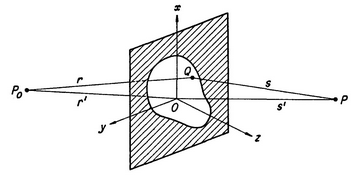
\includegraphics[width=0.4\textwidth]{Diagrama.png}
\caption{Modelado de Rendija General} \label{fig:rejilla}
\end{figure}
\end{block}
Para efectos teóricos, se utiliza la formulación matemática presentada anteriormente. Para simulaciones y toma de datos, se realizan aproximaciones discretas tanto del modelado de la rendija como de la transformada de Fourier.
\end{frame}

%Montaje
\begin{frame}
\frametitle{Simulaciones Preliminares}
Antes de realizar medidas, se realizan simulaciones del mismo fenómeno. Se utiliza Ipython Notebook para este propósito.
\begin{block}{Consideraciones}
\begin{itemize}
\item Aproximaciones discretas: Transformada de Fourier "Rápida" y rendija como matriz.
\item El espacio completo es una matriz, con valor constante distinto de 0 en la rendija y 0 en lo demás.
\end{itemize}
\end{block}
De igual forma que para la toma de datos, se utiliza una rendija simple, una doble rendija y una rendija circular.
\end{frame}

%Imágenes relevantes para ilustrar los resultados obtenidos en las simulaciones realizadas.
\begin{frame}
\frametitle{Simulaciones Preliminares}
\begin{block}{Rendija Única Cuadrada}
\begin{figure}[H]
\centering
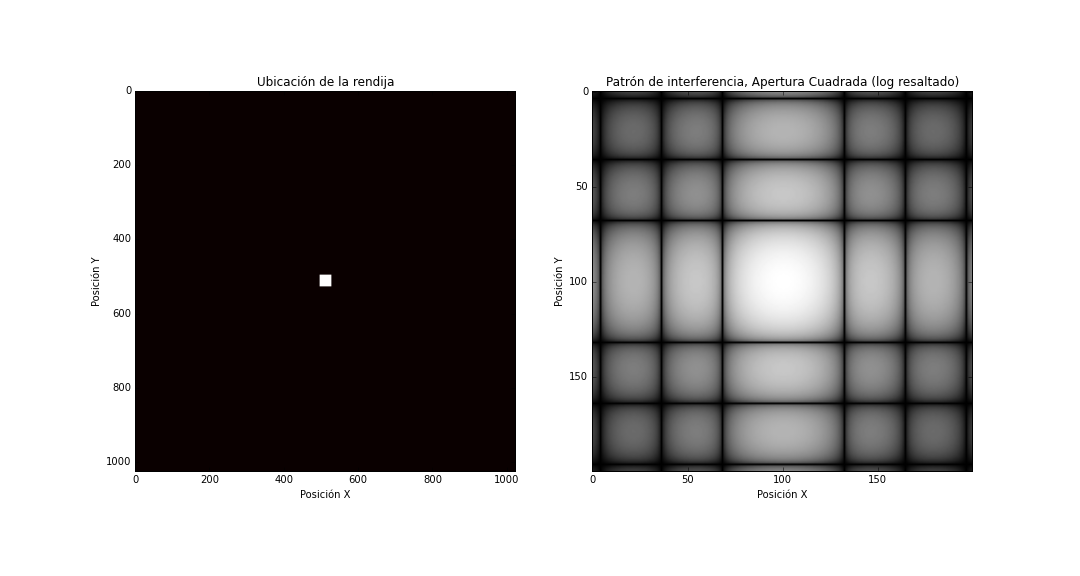
\includegraphics[width=0.55\textwidth]{Cuadrado.png}
\caption{Simulación de Rendija Cuadrada} \label{fig:rejillaCuad}
\end{figure}
\end{block}
\end{frame}
\end{document}

